\documentclass[]{beamer}
\usepackage{beamerthemesplit}
\usepackage{graphics,epsfig}
\usepackage{pstricks}
\usepackage{graphicx}
\usepackage{hyperref}
\usepackage{subfigure}
\usepackage{listings}
\usepackage{multirow}
\usepackage{xspace}
\usepackage[absolute,overlay]{textpos}
\usepackage{tikz}
\usetikzlibrary{decorations}
\usetikzlibrary{decorations.pathmorphing}
\usetikzlibrary{shapes,arrows}
\setlength{\TPHorizModule}{1cm}
\setlength{\TPVertModule}{1cm}


\mode<presentation>
{ \usetheme{Boadilla}
  \setbeamercovered{transparent}
  \setbeamertemplate{items}[circle]
  \setbeamertemplate{theorems}[numbered]
  \setbeamertemplate{footline}[frame number]
}
 
%\useinnertheme[shadow=true]{rounded}
\useoutertheme{shadow}
\usecolortheme{whale}

\newcommand\blfootnote[1]{
  \begingroup
  \renewcommand\thefootnote{}\footnote{#1}
  \addtocounter{footnote}{-1}
  \endgroup
}

\mode
<all>

\title{Programming in C}
\author{Wan-Lei Zhao}

\makeatletter

\begin{document}
\begin{frame}
   \begin{center}
    \vspace{24pt}
    \Huge\textbf{Programming in C}\blfootnote{Email: wlzhao@xmu.edu.cn, copyrights are fully reserved by the author.}\\
     %\Huge{Lecture 9: Operations on File}
     \begin{figure}
     	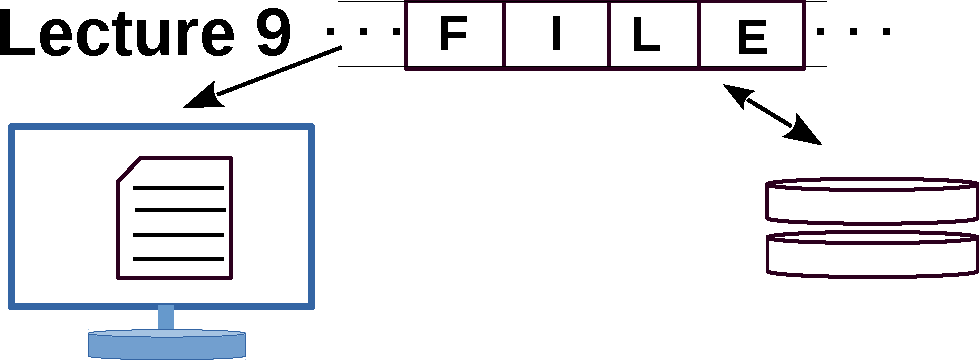
\includegraphics[width=0.6\linewidth]{figs/file_symb.pdf}
     \end{figure}
    \vspace{36pt}
  \end{center}
  \begin{align*}
   \vspace{18pt}
      \large{\mbox{Lecturer:}~Dr.~\mbox{Wan-Lei~~Zhao}} \\
      \large{Spring~~Semester~~2022} \\
   \vspace{30pt}
  \end{align*}
\end{frame}

\input{temps.tex}
\input{files.tex}
\section{}

\end{document}
